% Тип документа
\documentclass[a4paper,12pt]{extarticle}

% Шрифты, кодировки, символьные таблицы, переносы
\usepackage{cmap}
\usepackage[T2A]{fontenc}
\usepackage[utf8x]{inputenc}
\usepackage[russian]{babel}

% Это пакет -- хитрый пакет, он нужен но не нужен
\usepackage[mode=buildnew]{standalone}

\usepackage
	{
		% Дополнения Американского математического общества (AMS)
		amssymb,
		amsfonts,
		amsmath,
		amsthm,
		physics,
		% misccorr,
		% 
		% Графики и рисунки
		wrapfig,
		graphicx,
		subcaption,
		float,
		tikz,
		tikz-3dplot,
		caption,
		csvsimple,
		color,
		booktabs,
		pgfplots,
		pgfplotstable,
		geometry,
		% 
		% Таблицы, списки
		makecell,
		multirow,
		indentfirst,
		%
		% Интегралы и прочие обозначения
		ulem,
		esint,
		esdiff,
		% 
		% Колонтитулы
		fancyhdr,
	}  

\usepackage{xcolor}
\usepackage{hyperref}

 % Цвета для гиперссылок
\definecolor{linkcolor}{HTML}{000000} % цвет ссылок
\definecolor{urlcolor}{HTML}{799B03} % цвет гиперссылок
 
\hypersetup{pdfstartview=FitH,  linkcolor=linkcolor,urlcolor=urlcolor, colorlinks=true}
% Обводка текста в TikZ
\usepackage[outline]{contour}

% Увеличенный межстрочный интервал, французские пробелы
\linespread{1.3} 
\frenchspacing 

 
\usetikzlibrary
	{
		decorations.pathreplacing,
		decorations.pathmorphing,
		patterns,
		calc,
		scopes,
		arrows,
		fadings,
		through,
		shapes.misc,
		arrows.meta,
		3d,
		quotes,
		angles,
		babel
	}


\tikzset{
	force/.style=	{
		>=latex,
		draw=blue,
		fill=blue,
				 	}, 
	%				 	
	axis/.style=	{
		densely dashed,
		blue,
		line width=1pt,
		font=\small,
					},
	%
	th/.style=	{
		line width=1pt},
	%
	acceleration/.style={
		>=open triangle 60,
		draw=magenta,
		fill=magenta,
					},
	%
	inforce/.style=	{
		force,
		double equal sign distance=2pt,
					},
	%
	interface/.style={
		pattern = north east lines, 
		draw    = none, 
		pattern color=gray!60,
					},
	cross/.style=	{
		cross out, 
		draw=black, 
		minimum size=2*(#1-\pgflinewidth), 
		inner sep=0pt, outer sep=0pt,
					},
	%
	cargo/.style=	{
		rectangle, 
		fill=black!70, 
		inner sep=2.5mm,
					},
	%
	caption/.style= {
		midway,
		fill=white!20, 
		opacity=0.9
					},
	%
	}

\newenvironment{tikzpict}
    {
	    \begin{figure}[htbp]
		\centering
		\begin{tikzpicture}
    }
    { 
		\end{tikzpicture}
		% \caption{caption}
		% \label{fig:label}
		\end{figure}
    }


\newcommand{\vbLabel}[3]{\draw ($(#1,#2)+(0,5pt)$) -- ($(#1,#2)-(0,5pt)$) node[below]{#3}}
\newcommand{\vaLabel}[3]{\draw ($(#1,#2)+(0,5pt)$) node[above]{#3} -- ($(#1,#2)-(0,5pt)$) }

\newcommand{\hrLabel}[3]{\draw ($(#1,#2)+(5pt,0)$) -- ($(#1,#2)-(5pt,0)$) node[right, xshift=1em]{#3}}
\newcommand{\hlLabel}[3]{\draw ($(#1,#2)+(5pt,0)$) node[left, xshift=-1em]{#3} -- ($(#1,#2)-(5pt,0)$) }



\newcommand\zi{^{\,*}_i}
\newcommand\sumn{\sum_{i=1}^{N}}

\tikzset{
	coordsys/.style={scale=1.8,x={(1.1cm,-0cm)},y={(0.5cm,1cm)}, z={(0cm,0.8cm)}},
	coordsys/.style={scale=1.5,x={(0cm,0cm)},y={(1cm,0cm)}, z={(0cm,1cm)}}, 
	coordsys/.style={scale=1.5,x={(1cm,0cm)},y={(0cm,1cm)}, z={(0cm,0cm)}}, 
}

\usepgfplotslibrary{units}


% Draw line annotation
% Input:
%   #1 Line offset (optional)
%   #2 Line angle
%   #3 Line length
%   #5 Line label
% Example:
%   \lineann[1]{30}{2}{$L_1$}

\newcommand{\lineann}[4][0.5]{%
    \begin{scope}[rotate=#2, blue,inner sep=2pt, ]
        \draw[dashed, blue!40] (0,0) -- +(0,#1)
            node [coordinate, near end] (a) {};
        \draw[dashed, blue!40] (#3,0) -- +(0,#1)
            node [coordinate, near end] (b) {};
        \draw[|<->|] (a) -- node[fill=white, scale=0.8] {#4} (b);
    \end{scope}
}

\newcommand{\lineannn}[4][0.5]{%
    \begin{scope}[rotate=#2, blue,inner sep=2pt, ]
        \draw[dashed, blue!40] (0,0) -- +(0,#1)
            node [coordinate, near end] (a) {};
        \draw[dashed, blue!40] (#3,0) -- +(0,#1)
            node [coordinate, near end] (b) {};
        % \draw[color=white, color=blue] (a) -- node[fill=white, scale=0.8] {#4} (b);
        \draw[->|] (a)++(-0.3,0) -- (a);
        \draw[->|] (b)++(0.3,0) coordinate (xx) -- (b);
        \draw (xx) node[fill=white, scale=0.8, right] {#4};
    \end{scope}
}

% Круговая стрелка относительно центра (дуга из центра)
\tikzset{
  pics/carc/.style args={#1:#2:#3}{
    code={
      \draw[pic actions] (#1:#3) arc(#1:#2:#3);
    }
  },
  dash/.style={
  	dash pattern=on 5mm off 5mm
  }
}

% Среднее <#1>
\newcommand{\mean}[1]{\langle#1\rangle}

\pgfplotsset{
    % most recent feature set of pgfplots
    compat=newest,
}

% const прямым шрифтом
\newcommand\ct[1]{\text{\rmfamily\upshape #1}}
\newcommand*{\const}{\ct{const}}


\usepackage[europeanresistors,americaninductors]{circuitikz}

% Style to select only points from #1 to #2 (inclusive)
\pgfplotsset{select/.style 2 args={
    x filter/.code={
        \ifnum\coordindex<#1\def\pgfmathresult{}\fi
        \ifnum\coordindex>#2\def\pgfmathresult{}\fi
    }
}}


\usepackage{array}
\usepackage{pstool}


%%%%%%%%%%%%%%%%%%%%%%%%%%%%%%%%%%%%%%%%%%%%%%%%%
\makeatletter
\newif\if@gather@prefix 
\preto\place@tag@gather{% 
  \if@gather@prefix\iftagsleft@ 
    \kern-\gdisplaywidth@ 
    \rlap{\gather@prefix}% 
    \kern\gdisplaywidth@ 
  \fi\fi 
} 
\appto\place@tag@gather{% 
  \if@gather@prefix\iftagsleft@\else 
    \kern-\displaywidth 
    \rlap{\gather@prefix}% 
    \kern\displaywidth 
  \fi\fi 
  \global\@gather@prefixfalse 
} 
\preto\place@tag{% 
  \if@gather@prefix\iftagsleft@ 
    \kern-\gdisplaywidth@ 
    \rlap{\gather@prefix}% 
    \kern\displaywidth@ 
  \fi\fi 
} 
\appto\place@tag{% 
  \if@gather@prefix\iftagsleft@\else 
    \kern-\displaywidth 
    \rlap{\gather@prefix}% 
    \kern\displaywidth 
  \fi\fi 
  \global\@gather@prefixfalse 
} 
\newcommand*{\beforetext}[1]{% 
  \ifmeasuring@\else
  \gdef\gather@prefix{#1}% 
  \global\@gather@prefixtrue 
  \fi
} 
\makeatother
%%%%%%%%%%%%%%%%%%%%%%%%%%%%%%%%%%%%%%%%%%%%%%%%%

\geometry		
	{
		left			=	2cm,
		right 			=	2cm,
		top 			=	3cm,
		bottom 			=	3cm,
		bindingoffset	=	0cm
	}

%%%%%%%%%%%%%%%%%%%%%%%%%%%%%%%%%%%%%%%%%%%%%%%%%%%%%%%%%%%%%%%%%%%%%%%%%%%%%%%



	%применим колонтитул к стилю страницы
\pagestyle{fancy} 
	%очистим "шапку" страницы
\fancyhead{} 
	%слева сверху на четных и справа на нечетных
\fancyhead[R]{\labauthors} 
	%справа сверху на четных и слева на нечетных
\fancyhead[L]{Отчёт по лабораторной работе №\labnumber} 
	%очистим "подвал" страницы
\fancyfoot{} 
	% номер страницы в нижнем колинтуле в центре
\fancyfoot[C]{\thepage} 

%%%%%%%%%%%%%%%%%%%%%%%%%%%%%%%%%%%%%%%%%%%%%%%%%%%%%%%%%%%%%%%%%%%%%%%%%%%%%%%

\renewcommand{\contentsname}{Оглавление}

\usepackage{tocloft}
% \renewcommand{\cftpartleader}{\cftdotfill{\cftdotsep}} % for parts
% \renewcommand{\cftsectiondotsep}{\cftdotsep}% Chapters should use dots in ToC
\renewcommand{\cftsecleader}{\cftdotfill{\cftdotsep}}
%\renewcommand{\cftsecleader}{\cftdotfill{\cftdotsep}} % for sections, if you really want! (It is default in report and book class (So you may not need it).
% ---------
% \newcommand{\cftchapaftersnum}{.}%
% \usepackage{titlesec}
% \titlelabel{\thetitle.\quad}
\usepackage{secdot}
\sectiondot{subsection}

\begin{document}

\def\labauthors{Войтович Д.А., Карусевич А.А., Разова А.А.}
\def\labgroup{430}
\def\labnumber{5}
\def\labtheme{Апериодический усилитель}
\renewcommand{\vec}{\mathbf}
\renewcommand{\Re}{\operatorname{Re}}
\renewcommand{\Im}{\operatorname{Im}}
\renewcommand{\phi}{\varphi}
\renewcommand{\hat}{\widehat}

\begin{titlepage}

\begin{center}

{\small\textsc{Нижегородский государственный университет имени Н.\,И. Лобачевского}}
\vskip 1pt \hrule \vskip 3pt
{\small\textsc{Радиофизический факультет}}

\vfill

{\Large Отчет по лабораторной работе №\labnumber\vskip 12pt\bfseries \labtheme}
	
\end{center}

\vfill
	
\begin{flushright}
	{Выполнили студенты \labgroup\ группы\\ \labauthors}%\vskip 12pt Принял:\\ Менсов С.\,Н.}
\end{flushright}
	
\vfill
	
\begin{center}
	Нижний Новгород, \the\year
\end{center}

\end{titlepage}



%\tableofcontents
\newpage

\section{Теоретическая часть}
\subsection{Цель работы}
Исследование транзисторных апериодических усилителей с общим эмиттером (ОЭ) и общим коллектором (ОК).

\subsection{Назначение устройства}
Основным назначением усилителя является увеличение мощности электрических колебаний без изменения их формы. Кроме того, усилитель часто используется для развязки каскадов или их согласования.

\subsection{Область использования}
Усилители электрических колебаний имеют широкое и разнообразное применение: в радиосвязи и радиовещании, телевидении, звуковом кино, устройствах записи и воспроизведения звука, дальней проводной связи, измерительной аппаратуре, а также в телемеханике, автоматике, электронно-вычислительных машинах, аппаратуре исследования космического пространства и т.д.

\subsection{\textbf{Принципы работы усилителя}}
Качественные показатели усилителя во многом определяются режимом его работы. Под режимом работы понимается совокупность токов и напряжений в схеме, определяющих положение «точки покоя», т.е. состояние схемы до подачи на ее вход управляющего (входного) колебания.

При работе с сильными сигналами (обычно это при $U_{\text{вх}}>10$мВ) выбирают ту область статических характеристик транзистора, которая обеспечивает получение заданной максимальной амплитуды тока, напряжения или мощности при допустимой величине
нелинейных искажений и, по возможности, небольшом расходе энергии источника питания. Этим требованиям и должен подчиняться выбор режима работы. Выбор несколько различается в зависимости от того, какой эффект на выходе усилителя желательно получить, и в зависимости от типа усиливаемых сигналов.

Если необходимо обеспечить заданную амплитуду выходного тока $I_m$ в низкоомной нагрузке, то режим выбирают следующим образом. Тип используемого транзистора выбирается с таким расчетом, чтобы его максимально допустимая величина коллекторного тока удовлетворяла условию $i_km\geqslant 2I_m$ при симметричных биполярных сигналах и $i_km>I_m$ при однополярных сигналах.

\begin{figure}[h]
	\centering
	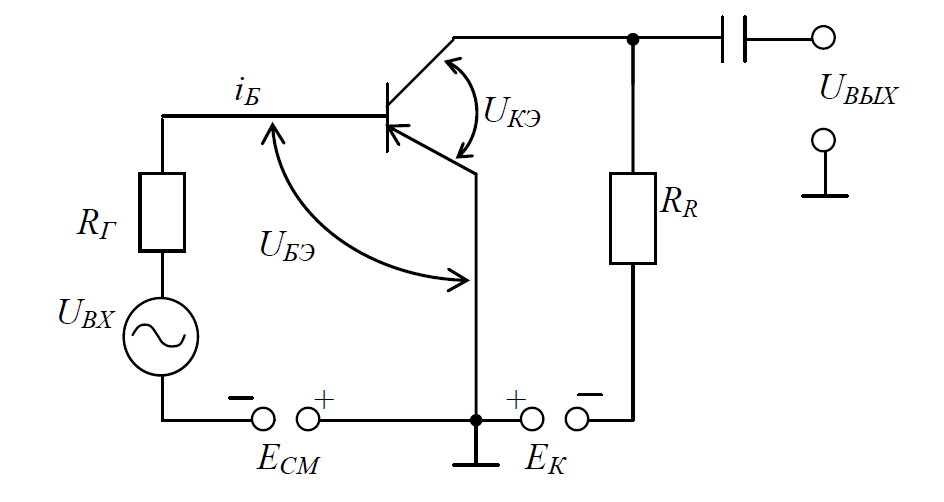
\includegraphics[width=0.5\linewidth]{fig/fig1}
	\caption{}
	\label{fig:1}
\end{figure}

В данной работе выбран транзистор МП41А.

\subsection{\textbf{Усилитель с общим эмиттером}}
В усилительных устройствах наиболее часто транзистор используется в схеме с общим эмиттером (ОЭ). В этой схеме (Рис.\ref{fig:1}) входным током является ток базы. Постоянная оставляющая тока базы задается величиной напряжения смещения $E_{\text{Б}}$, переменная составляющая создается источником сигнала $U_{\text{ВХ}}$ с внутренним сопротивлением $R_{\text{Г}}$. Выходным током называют ток коллектора. В его составе содержатся постоянная составляющая, определяемая начальным током базы и напряжением источника питания $E_{\text{К}}$, и переменная составляющая, пропорциональная управляющему напряжению $U_{\text{ВХ}}$. В реальной схемотехнике используются схемы усилителей, отличающиеся от схемы рис.\ref{fig:1} по ряду признаков. Рассмотрим простейшую из них (Рис.\ref{fig:2}):

\begin{figure}[h]
	\centering
	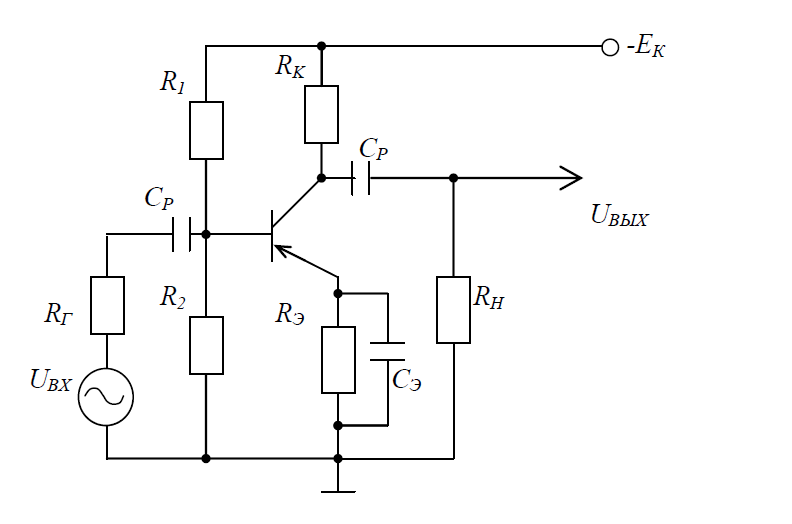
\includegraphics[width=0.5\linewidth]{fig/fig2}
	\caption{}
	\label{fig:2}
\end{figure}

Во-первых, в этой схеме отсутствует источник смещения $E_{\text{СМ}}$. Необходимое напряжение смещений создается за счет делителя напряжения $R_1$ и $R_2$, который, с учетом напряжения на резисторе $R_{\text{Э}}$, обеспечивает требуемое по величине и знаку постоянное напряжение на переходе база – эмиттер, и, следовательно, требуемое значение постоянной составляющей тока базы.

Во-вторых, в схему включены разделительные конденсаторы $C_p$, предназначенные для устранения влияния источника сигнала и внешней нагрузки $R_H$ на режим работы каскада. Конденсатор $C_p$ на входе совместно с входным сопротивлением каскада образует частотно – зависимый делитель, который уменьшает общий коэффициент усиления усилителя на нижних частотах. Аналогично учитывается влияние делителя $C_p$ и $R_H$. 

В-третьих, в схему включена цепочка $R_{\text{Э}}$ $C_{\text{Э}}$, предназначенная для температурной стабилизации режима  усилителя. Дело в том, что с повышением температуры окружающей среды в транзисторах наблюдается тепловой сдвиг вольт – амперных характеристик и, как следствие, изменение режима усилителя. Для снижения отрицательных последствий теплового сдвига в транзисторных усилителях реализуется термостабилизация режима. В ее основу положен механизм отрицательной обратной связи.

Термостабилизирующую роль $R_{\text{Э}}$, как элемента отрицательной связи можно описать на качественном уровне следующим образом. Пусть при начальной температуре среды ток базы равен $i_{\text{Б0}}$, напряжение смещения $U_{\text{Б0}}$, постоянная составляющая тока коллектора $i_{\text{K0}}$. С ростом температуры происходит тепловой сдвиг характеристик, в результате чего коллекторный ток получит приращение $\Delta i_{Kn}$. Это вызовет приращение напряжения на $R_{\text{Э}}$, равное $\Delta i_{Kn}R_{\text{Э}}$ . На эту же величину изменится смещение $U_{\text{Б0}}-\Delta i_{Kn}R_{\text{Э}}$, что приведет к уменьшению тока базы и к соответствующему уменьшению тока коллектора. Рабочая точка будет смещена к исходному положению, т.е. стабилизирована. Если емкость $C_{\text{Э}}$ отсутствует, то отрицательная обратная связь через $R_{\text{Э}}$ приведет к снижению усиления каскада. Чтобы избежать этого, сопротивление $R_{\text{Э}}$ шунтируют большой емкостью $C_{\text{Э}}$, что сохраняет отрицательную обратную связь только по постоянному току.

\end{document}

